\section{Introduction}\label{sec:intro}

\begin{figure}
  \centering
  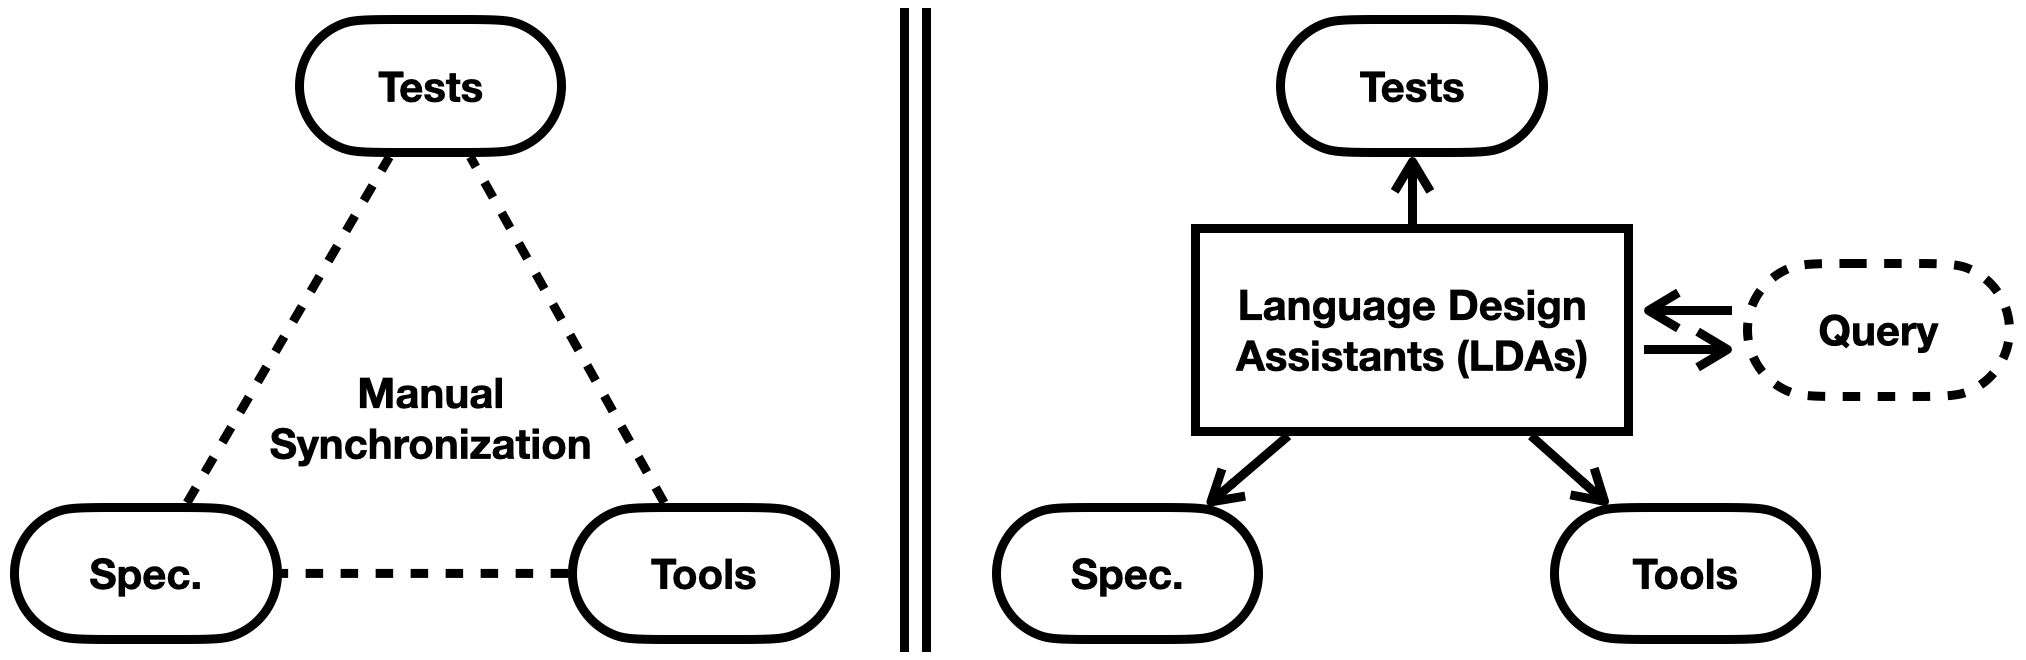
\includegraphics[width=\columnwidth]{img/lda.png}
  \caption{A manual approach (left) and a tool-oriented approach with language
    design assistants (right) with three language components: specifications,
  conformance tests, and language-based tools.}
  \label{fig:lda}
  \vspace*{-.5em}
\end{figure}

In the beginning, JavaScript was a scripting language designed in a ten-day
hack. However, it has become a de facto Web standard and eventually becomes one
of the dominating programming languages in various fields. For example,
Node.js\footnote{https://nodejs.org/} introduced full-stack JavaScript by
supporting server-side programming, and JavaScript has recently begun to be used
even in embedded systems and microcontrollers for the Internet of
Things\footnote{https://www.espruino.com/}. Furthermore, according to the annual
report of GitHub\footnote{\url{https://octoverse.github.com/}}, JavaScript has
consistently been the most popular programming language based on the number of
contributors to GitHub projects.

Recently, JavaScript has rapidly evolved with a yearly release cadence and open
development process. In 2015, The Ecma Technical Committee 39 (TC39) decided to
annually release ECMAScript, the standard specification for JavaScript, with a
massive update in ECMAScript 6 (ES6, 2015)~\cite{es6}. Therefore, six more
versions from ES7 to ES12 have already been released since 2015. Moreover, they
published the specification as an open-source project in a GitHub repository to
quickly adapt users' demands to the language.

In this fast-evolving nature of JavaScript, the need for \textit{language design
assistants} has grown to understand the current language semantics and to update
it with new language features in a tool-based approach. In the early 2000s,
\citet{lda} first presented the concept of language design assistants, and
several researchers actualized it in tools such as LISA~\cite{lisa} and
$\asfsdf$~\cite{asf-sdf, meta-env}. As described in Figure~\ref{fig:lda}, they
bridge the gap between three language components: specifications, conformance
tests, and language-based tools (e.g., parsers, interpreters, and compilers) by
automatically generating them from the language semantics. Moreover, they
provide query-based interactions to language designers for better understanding.
However, only small-size domain-specific languages are their targets due to
their low expressive power. On the other hand, several tools recently have been
presented towards language design assistants for JavaScript in academia and
industry. For example, JSExplain~\cite{jsexplain}, Narcissus~\cite{narcissus},
and engine262~\cite{engine262} are reference interpreters that closely follow
writing styles of ECMAScript, and they provide debugger-style support.
$\jiset$~\cite{jiset} is a tool to compile ECMAScript to an executable
specification. $\jest$~\cite{jest} is an extension of $\jiset$ to synthesize
conformance tests, and $\jstar$~\cite{jstar} is another extension that performs
type analysis for the specification.

However, existing tools for JavaScript language design assistants have two
limitations related to the \textit{understanding} and \textit{update} of
language semantics. First, they do not provide any automatic ways to focus on
target semantics for better comprehension. JavaScript language designers often
want to understand specific language semantics in the revision process. However,
existing tools do not provide mechanized methods; thus, finding related parts
manually in the specification or conformance tests is tedious. For example,
while reference interpreters and $\jstar$ visualize execution states and type
information, respectively, in the specification, they cannot localize parts in
the specification or conformance tests related to the target semantics. Second,
they manually or slowly synchronize three language components. For example,
there is no synchronization between reference interpreters with other language
components: ECMAScript and conformance tests. While $\jiset$ and $\jest$
automatically generate interpreters and conformance tests from ECMAScript, they
are appropriate for live language design because of the long time to extract
them from scratch for each semantics update.

In this paper, we present $\tool$, a \textit{live} language design assistant for
JavaScript with \textit{syntactic views}. Our tool extends $\jiset$ and $\jest$
to automatically synchronize language components and visualize additional
information for better understanding. To alleviate problems in existing tools,
we present two different techniques for better understanding and fast update of
language semantics, respectively. First, our tool provides a way to enhance the
understanding of the target semantics using a syntactic view, an abstract syntax
tree containing abstracted nodes. It automatically reduces semantics and filters
out conformance tests depending on user-defined syntactic views. To reduce
semantics in ECMAScript, we augment a partial evaluation~\cite{peval,
peval-survey} with syntactic views. We utilize statistical information to find
test programs related to a given syntactic view. Second, $\tool$ quickly
synchronizes language components in the language design process. Unlike $\jiset$
and $\jest$, our tool first detects which parts of semantics are revised and
partially updates related parts in specifications, conformance tests, and
language-based tools.

Our contributions are as follows:
\begin{itemize}
  \item We present $\tool$, a live language design assistant for JavaScript with
    syntactic views. It automatically synchronizes three language components:
    specifications, conformance tests, and language-based tools.
  \item We introduce a way to enhance the understanding of the target semantics
    using user-defined \textit{syntactic views}, abstract syntax trees
    containing abstract nodes. We experimentally demonstrate its effectiveness
    with randomly selected syntactic views.
  \item Towards \textit{live} language designs, we present an approach to detect
    which parts of semantics are revised and partially update related parts in
    language components. We also evaluate how it efficiently propagates
    modification to language components with randomly modified semantics.
\end{itemize}
